\chapter{气候预测集合初值扰动方法设计}
\label{cha:china}
\section{当前初值集合方案存在的问题}

混沌系统的初值不确定性会导致系统模拟结果有巨大的差异。而气候系统模式中的初值误差也会因为在系统内的非线性叠加而导致模拟结果与真实气候状态相距甚远。当前的气候预测系统中的初值大多是经过同化后的相对准确的结果。即便如此,改进后的初值相对于真实的大气状态还是有一定的差别。此时为了更好地改进预测结果,初值集合方案被提出。它是通过对初值进行微小的扰动,用扰动后的多个初值,进行集合预报,用集合预报的结果来代替单一的预报结果。特别是针对受到初始条件不确定性影响很强的耦合模式而言,初值集合预报更加必要。集合预报的方式已经应用在各大气象预报中心,是提高气象预测系统预测性能的一个重要方法。但是由于前面提到的气候系统模式的高计算代价以及气候预测的模拟时间较长等原因,面向气候预测的初值集合方案研究还有所欠缺。

第一章中简单介绍了天气初值集合方法和现有的气候集合方法。其中 滞后平均法方法理论基础不是特别完备,奇异向量法(SVs)实现上相对困难且计算代价高。因此本文试图将增长模繁殖法(BGM)应用于国家气候中心的季节集合预报。本文将探讨与BCC-CSM当前正在使用的LAF集合方法相比,BGM方法是否可以提高短期气候预测技巧。本章接下来的结构安排如下。第2节介绍了BCC-CSM气候系统模式和面向气候预测的BGM集合方法。第3节介绍了试验设计和集合评价标准,第4节将BGM和LAF集合方法预测结果进行了评估。
%第4节介绍了结果。

\section{基于气候系统模式改进的增长模繁殖法}
\subsection{BCC-CSM气候系统模式介绍}
本文中所使用的气候系统模式是由我国国家气候中心开发的BCC-CSM2-MR~\cite{wu2019beijing},它参加了国际耦合模式比较计划第六阶段(CMIP6),是在参加过CMIP5的BCC-CSM1.1m~\cite{wu2013global,xiao2013introduction}和早期的季节气候预测系统~\cite{liu2014relationships,liu2015performance}的基础上改进的模式。BCC-CSM2-MR和BCC-CSM1.1m之间的主要差异是大气和陆面模块中的物理过程。在大气模型中,垂直层的层数从26层增加到了现在的46层,并且将从对流源产生的重力波阻力引入了平流层。此外,BCC-CSM2-MR还更新了大气中深对流和云的参数化方案,并且增添了气溶胶的间接影响。BCC-CSM2-MR的陆地部分是BCC-AVIM2.0,它是在早期版本BCC-AVIM1.0上的改进,包括积雪、植被和土壤冻融过程。BCC-CSM2-MR的海洋和海冰模型组件与BCC-CSM1.1m相同。海洋模型是模块化海洋模型版本4(MOM4),其垂直层数为40,由地球物理流体动力学实验室(GFDL)开发。海冰组件是由GFDL开发的海冰模拟器(SIS)。海洋和海冰模型的水平分辨率为1$^\circ$经度,1/3$^\circ$纬度。与BCC-CSM1.1m相比,新的BCC-CSM2-MR在模拟平流层准两年振荡(QBO),东亚降水和地面气温的长期趋势方面取得了显著的进步~\cite{wu2019beijing}。BCC-CSM2-MR目前正在调研进一步提升季节气候预报技巧的方法,为新一代BCC-CSM气候预报系统做准备。
\subsection{面向气候预测的增长模繁殖法初值扰动集合设计}

增长模繁殖法首先在天气初值集合扰动方法中被提出。它的主要思路是利用对初始场的随机扰动来模拟初始场的误差,并通过反复将扰动在模式中进行繁殖而获取快速增长的误差,以此作为集合预报的初始场的最终扰动~\cite{toth1997ensemble}。其一般流程如下所示:

(1) 初始场上叠加(扣除)随机扰动

(2) 将扰动场和控制场一起往前积分一段时间

(3) 获取扰动场和控制场的差,作为此繁殖循环的增长模

(4) 调整增长模尺度使其与初始扰动在均方根意义上相当,将调整后的增长模作为下一次繁殖循环的扰动

(5) 重复2-4步骤,直到增长模的增长率饱和,此时获得的最终扰动,即为集合预报初始场的最终扰动。

增长模繁殖法的示意图如~\ref{fig:bgm}所示:
\begin{figure}[H] % use float package if you want it here
  \centering
  \includegraphics[scale=0.8]{figures/bgm.jpg}
  \caption{BGM流程示意图}
  \label{fig:bgm}
\end{figure}

研究表明,在增长模繁殖法中的关键技术主要有以下三点~\cite{郑峰2008集合预报初值扰动在天气预报中的应用研究进展}:
(1) 繁殖循环的每一个循环的长度是多少,总繁殖周期是多长;
(2) 初始扰动该如何选择;
(3) 如何选择增长模的动态调整方法。

在天气集合预报中每一个繁殖循环的长度通常为6h或者12小时,增长模增长率大约在3-4天之后就会饱和~\cite{toth1997ensemble,zhang2010beating}。而如此之快的饱和速度对于气候预报明显是不适合的,因为在气候预报中不仅有快速变化的物理过程,还有相对慢变化的过程,增长模的增长率过早地达到饱和,会使得慢变化过程中的特征和误差没有被完全捕捉。另外有研究表明不同的动力框架应选取不同的繁殖循环长度,且在耦合模式中需要更长的繁殖循环长度~\cite{yang2006enso,baehr2013ensemble}。根据以上的介绍,针对于BCC-CSM气候系统模式,本文通过实验调整,找到了最优的繁殖循环时间为每5天为一个循环,共繁殖4次,总繁殖周期为20天。增长率的计算公式将在下面和动态调整方法一起介绍。
增长率随繁殖循环变化图如~\ref{fig:bred cycle}。
\begin{figure}[H] % use float package if you want it here
  \centering
  \includegraphics[scale=0.5,trim=0 0 0 30,clip]{breeding_cycle.png}
  \caption{增长率随繁殖循环变化图}
  \label{fig:bred cycle}
\end{figure}

初始扰动的获取,在天气中一般的选择是扰动某单个或者多个变量,使其尺度与模式初始场预报1小时所产生的误差在同一等级。而在气候中这一做法显然不合理。其主要原因是由于气候预报主要关注的是较长时间尺度的气候特征,在1小时预报尺度上的误差很大,与真实的初始场可能存在的误差差距很大。本文这里的做法是对初始场随机扰动使其与全球观测误差分布尺度相当。另外为了使得集合预报在多个变量上都取得较好的结果,本文选择的扰动变量有纬向风,径向风,温度,相对湿度。模式初始场是一个瞬时文件,本文选择的气候变量都是三维的(经度,纬度,垂直高度)变量,扰动也是三维的随机扰动。这样能够对不同垂直层的气候都有一个微小的扰动,让扰动场更有可能包含真实的气候初始场。

增长模动态调整方法通常是将增长调整到与初始扰动均方根在同一个量级,此处面向气候的BGM方法与天气中保持一致。这个操作的意义在于使得快速增长的误差被保留而慢增长的误差在循环中逐渐被忽略。另外扰动变量的均方根的计算为所有垂直层的平均均方根。

前文介绍了面向气候预测的BGM方法的关键技术,接下来将叙述方法的实现细节。方法的实现共分为以下三个主要部分:初始扰动生成,繁殖循环流程建立和并行集合预测提交。其中初始扰动的获取利用NCL(NCAR Command Language)和NCO(netCDF Operators)来实现的,繁殖循环流程建立和并行集合预测提交则都是利用Shell脚本来控制的。

初始扰动部分生成了4对扰动,让每个初始扰动并行进入繁殖循环流程,它包括气候系统模式的自动匹配提交,增长模的获取以及动态调整因子和增长率的计算等模块。由上文可知,在获取初始扰动场之后要将扰动场和控制预报一起往前报一个繁殖循环长度。这里通过Shell脚本自动更改气候系统模式提交的日期,运行的时长以及所需要的初始场等信息。在判断扰动预报和控制预报一个繁殖循环都运行完之后将扰动预报和控制预报相减获取增长模。按照下述公式计算增长率和动态调整因子。假设初始扰动为$p_0$,它在均方根意义上的大小可由以下公式表达。
\begin{align}
&  { E } \left( p _ { 0 } \right) = ({\frac{ \sum _ { i = 1 } ^ { N } p _ { 0 i } ^ { 2 }}{N}})^ { 1 / 2 } 
\end{align}
其中$N$为全球格点数,$p_{0i}$为i格点上的扰动大小。设第$t$步繁殖循环之后所获得的扰动场如下所示:
\begin{align}
& p _ { t } ^ { \prime } = f _ { t } ^ { \mathrm { perb } } - f _ { t } ^ { \mathrm { cntl } } 
\end{align}
其中$f _ { t } ^ { \mathrm { perb } }$为$t$时刻的扰动预报场,$f _ { t } ^ { \mathrm { cntl } }$为$t$时刻控制预报场。则$t$时刻的动态调整系数如下所示:
\begin{align}
& { rescaleFac } = \frac { E \left( p _ { 0 } \right) } { E \left( p _ { 1 } \right) } 
\end{align}
增长率的计算公式如下:
\begin{align}
& growthRate _ { t } = \frac { E \left( p _ { t } ^ { \prime } \right) } { E \left( p _ { t } \right) } = \frac { E \left( p _ { 0 } \right) } { resaleFac _ { t } E \left( p _ { t } \right) } 
\end{align}
其中$E \left( p _ { t } \right) = E \left( rescaleFac _ { t - 1 } p _ { t - 1 } ^ { \prime } \right)$,为$t-1$步输出模经过调整得到的第$t$步循环的输入模。

当所有的繁殖循环完成,扰动场都已准备完毕,将其加到起始预报当日的初始场上,面向气候的增长模繁殖法共获得了8个扰动场,此时利用Shell脚本控制所有正扰动预报和负扰动预报以及控制预报的提交,得到9个集合预报的结果。整合以上流程,面向气候预测的BGM初值集合预报流程示意图如图~\ref{fig:bgm ensem fore}所示。

\begin{figure}[H] % use float package if you want it here
  \centering
  \includegraphics[scale =0.37]{figures/初值集合预报示意图.pdf}
  \caption{BGM初值集合预报示意图(d为天数,m为月份)}
  \label{fig:bgm ensem fore}
\end{figure}

\section{试验设计与集合评价标准}
为了证明本文所提出的面向气候的BGM方法的有效性,下面将此BGM方法与国家气候中心正在使用的面向气候的LAF进行对比。此LAF方法集合成员的初值选取分别相对滞后3天。比如说第一个成员相对于控制预报滞后3天,第二个成员则滞后6天,依次类推。此方法所依赖的原理是相近的天数的初值相似程度高,并且有一定的离散度。接下来将详细介绍两种集合方法的试验设计和评价指标。

1. 试验设计。回报试验的时间选在2000年-2014年,分别从每年的5月1日报到8月31日。两种集合方法的成员数目相同,都是8个扰动预报加一个控制预报。本文所评价的气候变量及其观测数据的来源见表~\ref{tab:eva varibles}。

\begin{table}[htb]
\centering
\caption{气候变量及其对应的观测数据}  
\begin{tabular}{lll}
\toprule[1.5pt]
变量名称 & 变量含义 & 观测\\  
\hline  
T850     & 850hPa Temperature   & ERAI-Interim\\
    U850   & 850hPa zonal wind  & ERAI-Interim\\
    U200    & 200hPa zonal wind    & ERAI-Interim\\
    V850     & 850hPa meridional wind   & ERAI-Interim\\
    Z500     & 500hPa geopotential height  & ERAI-Interim \\
    PRECT & precipitation & GPCP \\
    TREFHT & surface air temperature(SAT) & ERAI-Interim\\
\bottomrule[1.5pt] 
\label{tab:eva varibles}
\end{tabular}  
\end{table}

2.集合评价指标。集合结果的评价一般应有两个方面,一是确定性预报的结果,即将集合成员的结果综合成一个确定的预报结果。二是概率性预报结果,即提供某一事件出现的可能性等。本章以确定性评价指标为主,概率性指标为辅对两种集合方法进行评比。

(1)确定性评价指标。这里的确定性预报结果仍使用的集合平均。衡量确定性预报结果的指标有RMSE(Root mean square error)、TCC(Temporal correlation coefficient)、离散度等。RMSE和TCC都是将集合平均结果与观测做对比以检验哪一组结果离观测更加接近。集合离散度计算的是集合本身的标准偏差,标准偏差越大则说明集合成员之间的差异大,集合平均的结果可信度越小,反之则反。通常预报员在进行确定性预报时要同时结合集合离散度和集合平均等结果共同作出决策。RMSE计算如公式~\ref{equ:RMSE}所示。
\begin{equation}
\label{equ:RMSE}
R M S E = \sqrt { \frac { \sum _ { i = 1 } ^ { N } \left(  w(i)  (  x _ { i } - f _ { i } ) \right) ^ { 2 } } { N } }
\end{equation}
其中$N$为预报格点总数,$x _ { i }$为$i$格点上的观测值,$f _ {  i }$是$i$格点上的模式预测值。$w(i)$为格点权重。RMSE用来衡量观测与预报之间的距离,距离越小,预报能力越强。
每个网格的TCC的计算如公式~\ref{equ:TCC i}。
\begin{equation}
\label{equ:TCC i}
T C C _ { i } =  \frac { \sum _ { j = 1 } ^ { M } \left( _ { X _ { i , j } } - \overline { x _ { i } } \right) \left( f _ { i , j } - \overline { f _ { i } } \right) } { \sqrt { \sum _ { j = 1 } ^ { M } \left( x _ { i , j } - \overline { x _ { i } } \right) ^ { 2 } } \times \sqrt { \sum _ { j = 1 } ^ { M } \left( f _ { i , j } - \overline { f _ { i } } \right) ^ { 2 } } }
\end{equation}
其中$x _ { i , j }$为$i$格点$j$时间上的观测,$x _ { i }$为$i$格点上的观测平均值。$ f _ { i , j }$为$i$格点$j$时间上的模式预测值,$f _ { i }$为$i$格点上的预测平均值。
若要计算区域或者全球平均时也需要考虑每个格点的权重。公式如下所示:
\begin{equation}
\label{equ:Rasfuc}
T C C = \frac { \sum _ { i = 1 } ^ { N } w(i) T C C _ { i } } { \sum _ { i = 1 } ^ { N } w(i) }
\end{equation}
其中$N$为格点总数,$w(i)$为格点权重。TCC指标能够在统计意义上较好地衡量每个格点的异常情况,得到完整的空间评分技巧分布。

(2)概率性评价指标。Brier评分是集合概率性评价的常用指标,其计算方法如公式~\ref{equ:Brier}所示:
\begin{equation}
\label{equ:Brier}
B S = \frac { 1 } { n } \sum _ { i = 1 } ^ { n } \left( f _ { i } - o _ { i } \right) ^ { 2 }
\end{equation}
其中,$n$为预报次数,$f _ { i }$是第$i$次预报的事件发生概率,$o _ { i }$为第$i$次观测的概率,如果事件发生,$o _ { i }$等于1,若没有发生,则为0。BS的结果在0-1之间,其值越小表明预测概率与观测越接近,预报技巧越高。

\section{增长模繁殖法集合预测效果评估}
为了更好地对BGM和LAF的结果进行分析比较,这里分别对两个集合确定性预报和概率性预报结果进行检测,确定性预报检测的流程如下所示。首先本文将计算RMSE和TCC指标,并画出全球空间分布图,从全球平均RMSE和TCC等指标本文能够初步判断两个集合的全球平均预报能力,空间分布图又提供了全球每个格点的情况,根据空间分布图本文能够对不同区域两种集合方法的预报能力有了进一步的认识。此时再利用TCC显著性检验挑出通过检验的区域,分析区域内集合预报技巧。此分析流程从总体到局部,详细的对集合结果做了多方位的评价,分析的输出为可视化的图形,直观且容易理解。

图~\ref{fig:global rmse}中分别展示了BGM和LAF集合预报的全球降水,地表温度、850hPa径向纬向风、500hPa位势高度、200hPa纬向风的全球平均分布的RMSE差,如果差小于0的话,则说明BGM集合方案的RMSE要小于LAF集合方案的RMSE,即BGM方法优于LAF方法。从图~\ref{fig:global rmse}(a)中可以看出两个集合方法对降雨的确定性预报差距不是很明显,除了在赤道太平洋区域略有变化。图~\ref{fig:global rmse}(b)中显示BGM预测的地表温度在亚洲东北部相对LAF有较为明显的提升。850hPa径向风在全球的中高纬度地区相比LAF有所提高,而850hPa纬向风和500hPa位势高度在北半球的大部分区域都有显著的改善。200Pha纬向风在北半球中纬度地区改善明显。从图中可以看出BGM方法相比LAF在预报后的第一个月中可以有效地减小对流层低层和高层纬向风以及对流层中层的位势高度的模型误差。

为了探索两个集合方法在起报随时间往后的月份(lead month)中表现情况,图~\ref{fig:global rmse lead time}中展示了两个集合方法的所有预报月份的200hPa纬向风、500hPa位势高度、850hPa经纬向风的全球平均RMSE。从图中可以看出BGM在这四个变量的预报的第一个月中都有明显的提升,且500hPa位势高度在所有预报月份中都相对LAF预测结果变好。

\begin{figure}[H] % use float package if you want it here
  \centering
  \includegraphics[scale=0.8,trim=1 50 1 75,clip]{Fig2_dif_rmse_May_diff_six.eps}
  \caption{BGM和LAF在5月的PRECT、SAT、U850、V850、Z500、U200的全球RMSE差异分布}
  \label{fig:global rmse}
\end{figure}

\begin{figure}[H] % use float package if you want it here
  \centering
  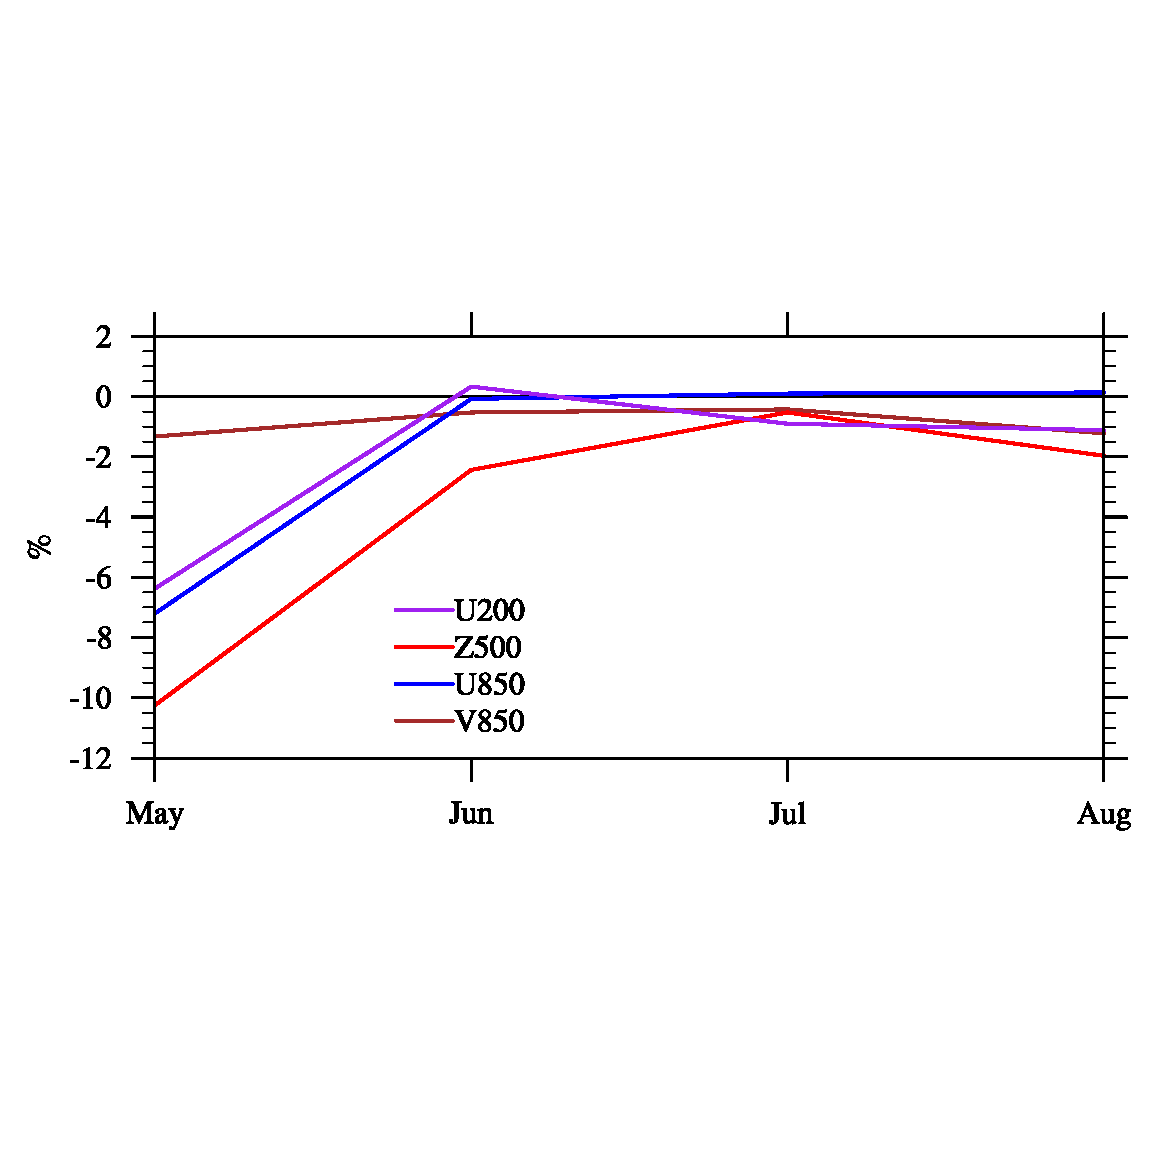
\includegraphics[scale=0.45,trim=1 110 1 150,clip]{figures/Fig3_dif_rmse_May_Aug_series.eps}
  \caption{BGM和LAF在5月到8月的U200、Z500、U850、V850全球平均RMSE差异}
  \label{fig:global rmse lead time}
\end{figure}

RMSE衡量的是观测值与预测值的相对差值,TCC则充分考虑两个集合预测结果在空间上的相似程度。从图~\ref{fig:TCC four vari}中可以看出在5月份所有变量在北半球大陆通过TCC显著性检验的区域都是BGM集合比LAF更多。对于850hPa径向风来说,BGM集合预报在中国北部,热带西太平洋比LAF集合预测的TCC更显著。对于850hPa纬向风BGM方法在欧洲和西太平洋相对LAF方法有所提升。而500hPa位势高度和200hPa纬向风在全球大部分区域BGM比LAF的TCC都要更好,尤其是在欧亚大陆。

\begin{figure}[H] % use float package if you want it here
  \centering
  \includegraphics[scale=0.7,trim=1 40 1 50,clip]{figures/Fig4_dif_cor_May_circulation.eps}
  \caption{5月V850、U850、Z500、U200的TCC空间分布(阴影区域置信水平高于90\%)}
  \label{fig:TCC four vari}
\end{figure}

\begin{figure}[H] % use float package if you want it here
  \centering
  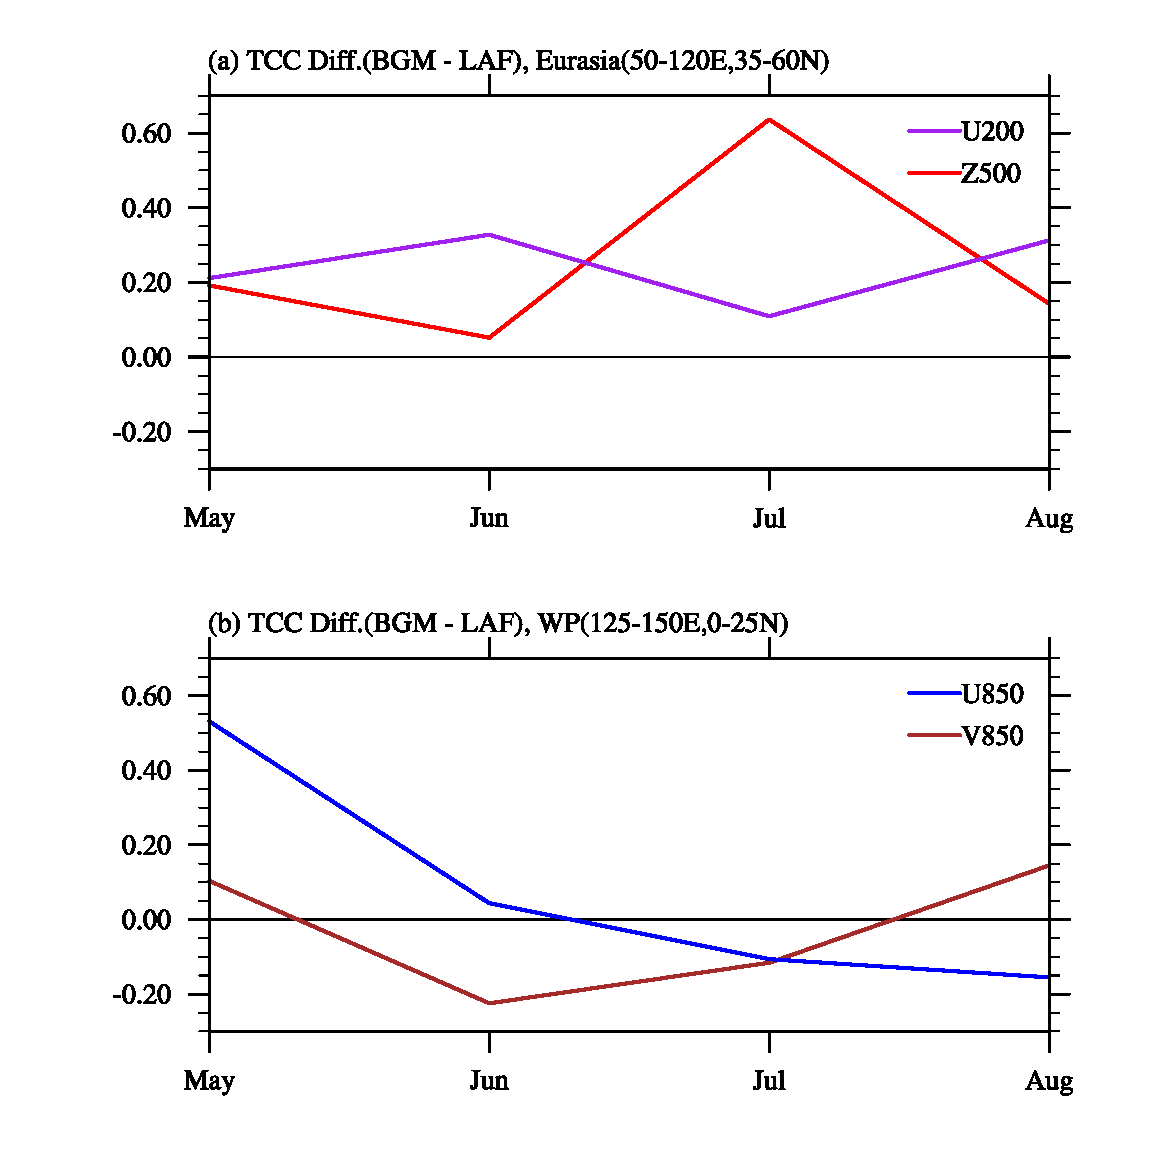
\includegraphics[scale=0.45,trim=1 10 1 16,clip]{figures/Fig5_dif_cor_May_Aug_series.eps}
  \caption{BGM和LAF在欧亚大陆和西太平洋区区域平均TCC差异}
  \label{fig:Tcc eura and wes pac}
\end{figure}

考虑到欧亚大陆中高层大气环流和西太平洋低层风对亚洲气候的影响,本文进一步关注U200和Z500在欧亚大陆(50$^\circ$-120$^\circ$E 35$^\circ$-60$^\circ$N)以及U850和V850在西太平洋(125$^\circ$-150$^\circ$E, 0-25$^\circ$N) 区域的平均TCC结果。

如图~\ref{fig:Tcc eura and wes pac}(a)所示,500hPa位势高度和200hPa纬向风在所有月份都变好明显。而在西太平洋区域850hPa经纬向风只在5月份BGM方法有所提升(图~\ref{fig:Tcc eura and wes pac}(b))。因此,BGM相对LAF集合方法对欧亚大陆对流层中上层环流的集合预测效果更好,影响时间更长。

\begin{figure}[H] % use float package if you want it here
  \centering
  \includegraphics[scale=0.8,trim=1 125 1 130,clip]{figures/Fig6_dif_cor_May_EA.eps}
  \caption{东亚地区降水和地表温度TCC}
  \label{fig:Tcc of ea pr and sat}
\end{figure}
欧亚大陆BGM方法预报技巧的提升说明了BGM可能对于地表气候的模拟有良好的效果。图~\ref{fig:Tcc of ea pr and sat}显示了BGM和LAF方法在亚洲降水和温度上的TCC空间分布图,从图中可以看出BGM相比LAF在亚洲东北部,中国北方和西太平洋区域预报能力更好。因此可以看出本文所设计的BGM方法是一种有效提升亚洲区域预报能力的方法。

本文选取亚洲西北区域(60$^\circ$-100$^\circ$E, 50$^\circ$-70$^\circ$N),亚洲东北(100$^\circ$-140$^\circ$E, 50$^\circ$-70$^\circ$N),中国北方(100$^\circ$-120$^\circ$E, 30$^\circ$-42$^\circ$N)以及西太平洋区域计算区域平均的降水(PR)和地表温度(SAT)从2000到2014年每年5月的时间序列。由图~\ref{fig:pre and sat corre}可知,BGM预测的亚洲西北部、华北和西太平洋5月降水年际变化较LAF预测的更符合观测结果(图~\ref{fig:pre and sat corre} a,c), 三个区域降水的时间相关系数分别为0.51、0.52和0.62,远高于LAF预报与观测的时间相关系数。BGM集合还在东亚北部、华北、西太平洋地区重现了更为合理的地表温度年际变化,相关系数别为0.62、0.82、0.47(图~\ref{fig:pre and sat corre} d,f)。它们都高于LAF集合预测与观测值之间的时间相关性。BGM集合预测的这些区域降水和地表温度能力的提高与欧亚大陆的Z500和U200以及西太平洋的U850和V850等大气环流的改善是一致的。

\begin{figure}[H] % use float package if you want it here
  \centering
  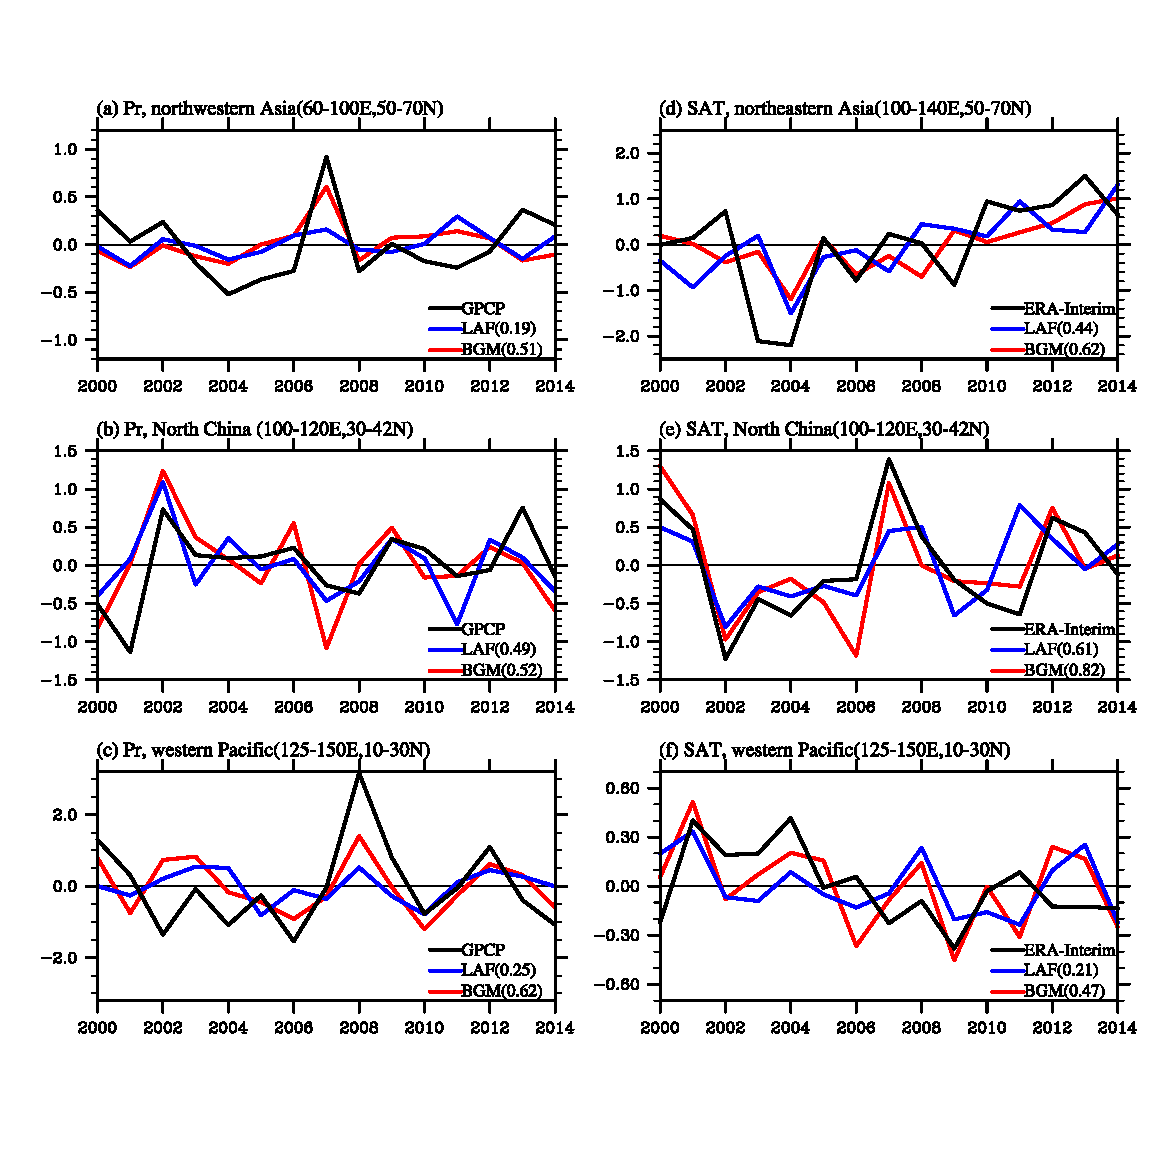
\includegraphics[scale=0.8,trim=1 50 1 30,clip]{figures/Fig8_May_BGM_LAF_2000_2014.eps}
  \caption{降水和地表温度异常相关系数}
  \label{fig:pre and sat corre}
\end{figure}

夏季亚洲气候的预测对于以一个月为主导时间的BCC-CSM季节预测系统来说仍然是一个挑战~\cite{liu2015performance}。如图~\ref{fig:summer pre and sat} a和b所示,LAF和BGM集合预测的东亚降水预测能力都较低。BGM和LAF集合方法在印度、阿拉伯海和中国南海的地表温度预报能力中都表现出了很高的水平,但在东亚大陆的预报水平却很低(图~\ref{fig:summer pre and sat} d,e)。

另外图~\ref{fig:BS}也分别展示了U200、Z500、U850和V850的概率性集合预报评测Brier评分的结果。结合图~\ref{fig:TCC four vari}和~\ref{fig:global rmse lead time}可以看出概率性预报评价方式Brier评分的结果与确定性集合方法中模拟结果优劣的趋势非常相似,U200、Z500、U850、V850四个变量都是第一个月BGM相对LAF变好趋势明显,Z500和V850变好的时间可以持续更长。因此在后续的集合评价中本文延续了确定性集合评价方法。

\begin{figure}[H] % use float package if you want it here
  \centering
  \includegraphics[scale=0.8,trim=1 120 1 130,clip]{figures/Fig7_dif_cor_JJA_EA.eps}
  \caption{夏季东亚地区降水和地表温度TCC}
  \label{fig:summer pre and sat}
\end{figure}
%其中U200,Z500,U850,V850的阈值选择为
\begin{figure}[H]
\centering
\begin{minipage}[t]{0.48\textwidth}
\centering
\includegraphics[width=8cm]{figures/brier-15-U200.pdf}
%\caption{DTLZ7 hypervolume}
\end{minipage}
\begin{minipage}[t]{0.48\textwidth}
\centering
\includegraphics[width=8cm]{figures/brier-15-Z500.pdf}
%\caption{DTLZ7 IGD}
\end{minipage}

\centering
\begin{minipage}[t]{0.48\textwidth}
\centering
\includegraphics[width=8cm]{figures/brier-15-U850.pdf}
%\caption{DTLZ7 hypervolume}
\end{minipage}
\begin{minipage}[t]{0.48\textwidth}
\centering
\includegraphics[width=8cm]{figures/brier-15-V850.pdf}
%\caption{DTLZ7 IGD}
\end{minipage}
\caption{U200,Z500,U850,V850全球平均BS评分}
\label{fig:BS}
\end{figure}
%[width=8cm]

\section{本章小结}

本章将BGM集合预测方法应用于BCC-CSM的季节气候预报。此面向气候的BGM方法每隔5天对分析误差进行重新调整,经过4个繁殖周期,分析误差的增长率达到饱和。扰动变量包括纬向风、经向风、温度和比湿度。从5月1日开始,对2000-2014年每年进行为期4个月的预测,BGM与每隔3天产生不同初始时延的LAF方法的对比结果表明,相对于LAF,BGM集合方法可以降低U200、V850、U850、Z500和U200在全球大部分地区第一个月(5月)的RMSE。U850和Z500的RMSE减小情况会持续整个夏天。与LAF集合方法相比,BGM预测的全球500hPa位势高度的RMSE在5月份平均下降10.2\%,在夏季平均下降1.7\%。从TCC的角度来看,BGM集合方法对欧亚大陆夏季5月份的U200和Z500具有较高的预测能力。西太平洋U850和V850的TCC技术仅在5月份有所提高。在亚洲和西太平洋地区,BGM集成预报降水和地表温度的TCC预报技巧在提前一个月时间内优于LAF方法。但是由于夏季气候的多变特性,BGM和LAF对夏季降水和地表温度的预测能力都较弱。综合以上结果,BGM方法比LAF方法更适合次季节的气候预测。
